\chapter{Experiments}
As mentioned in the previous chapter, the process of finding was an iterative one of running an experiment, analyzing the generated data, draw conclusions and then repeat the steps with a new experiments designed to amend the mistakes of the previous experiment. This chapter will go through each of these steps and explain the insights that were gained.

This chapter presents the flow of analysis as it was carried out, rather 

A summary and discussion of the results is found in chapter \ref{chapter:discussion}.


\section{D3}
In this experiment, the number of \ssmmnAgents and \scnAgents as well all the latency parameters were included in the individuals. The genetic algorithm was run for 1000 generations with a population size of 200. A total of 


This data set was generated by including all the model parameters concerning time latency as well as the number of agents into the individuals in the genetic algorithm. Due to the high number of variables, the data turned out to be difficult to analyze, as too many factors pertaining to the simultaneous change of several parameters influenced the fitness values. Thus, not many definitive results concerning the impact of time latency of market behavior were derived from this data set. The reason why it is still included in the thesis is that the data did provide hints on how to proceed with the analysis of the model. Furthermore, the data set proved useful for developing the tools used to analyze the data sets that were generated later, and hence this section is intended to illustrate the motivation for applying these tools.

Scatter plots of the fitness data before and after preprocessing were already shown in figure \ref{figure:scatter_log_transform}.

\begin{table}
	\centering
	\begin{tabular}{l|l}
	Dataset id & Parameters in genes\\
	\dthree & \sclatencymu, \sclatencys, \scnAgents, \scthinkmu, \scthinks, \sctimehorizonmu, \sctimehorizons, \scwaitTimeBetweenTradingmu, \scwaitTimeBetweenTradings, \ssmmlatencymu, \ssmmlatencys, \ssmmnAgents, \ssmmthinkmu, \ssmmthinks	
	\end{tabular}
\end{table}

Free parameters:

Data set \dthree was the first run of the genetic algorithm that actually produced something that looked like results. The following parameters were included in the genetic algorithm individuals:
\begin{center}
\sclatencymu, \sclatencys, \scnAgents, \scthinkmu, \scthinks, \sctimehorizonmu, \sctimehorizons, \scwaitTimeBetweenTradingmu, \scwaitTimeBetweenTradings, \ssmmlatencymu, \ssmmlatencys, \ssmmnAgents, \ssmmthinkmu, \ssmmthinks
\end{center}

Fixed parameters:




\begin{figure}
	%issue 15
	\centering
	\subcaptionbox{Evolution of \ssmmlatencymu and \sclatencymu}
	[0.49\linewidth]{\includegraphics[width=0.5\textwidth]{82_generation_plots/d3/latpars_mu.png}}
	\subcaptionbox{Evolution of \ssmmthinkmu and \scthinkmu}
	[0.49\linewidth]{\includegraphics[width=0.5\textwidth]{82_generation_plots/d3/thinkpars_mu.png}}
	\subcaptionbox{Evolution of \nmm and \nsc}
	[0.49\linewidth]{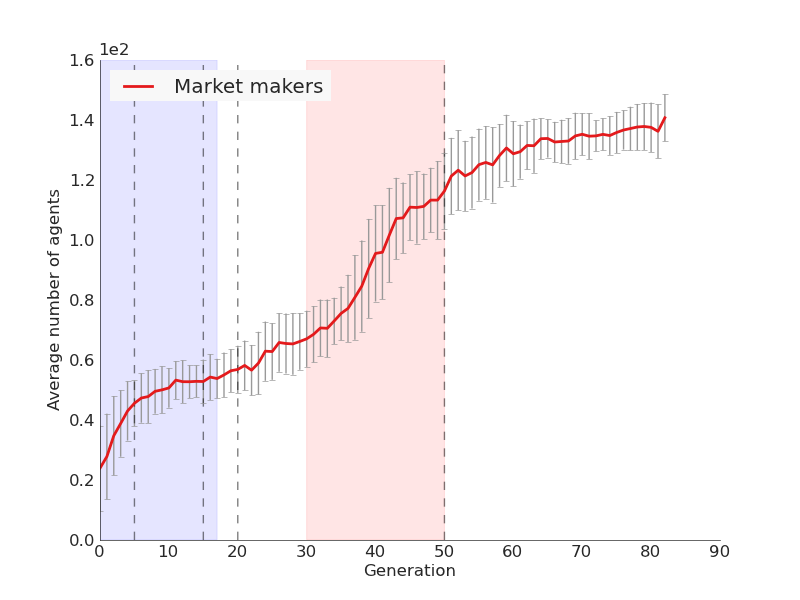
\includegraphics[width=0.5\textwidth]{82_generation_plots/d3/nAgents.png}}	\caption{Evolution of time delay parameters common both HFT agent types, and of the number of agents in experiment \dthree}\label{fig:d3_evolution_latpars_nAgents}
\end{figure}


\begin{figure}
	%issue 15
	\subcaptionbox{Evolution of \sctimehorizonmu}
	[0.49\linewidth]{\includegraphics[width=0.5\textwidth]{82_generation_plots/d3/sctimehorizon_mu.png}}
	\subcaptionbox{Evolution of \scwaitTimeBetweenTradingmu}
	[0.49\linewidth]{\includegraphics[width=0.5\textwidth]{82_generation_plots/d3/scwaittime_mu.png}}
	\caption{Evolution of chartist-specific strategy parameters in experiment \dthree}\label{fig:d3_evolution_thinkpars}
\end{figure}

\begin{figure}
	%issue 15
	\centering
	\subcaptionbox{Evolution of \roundstable}
	[0.49\linewidth]{\includegraphics[width=0.5\textwidth]{82_generation_plots/d3/round_stable.png}}
	\subcaptionbox{Evolution of \timetoreachnewfundamental}
	[0.49\linewidth]{\includegraphics[width=0.5\textwidth]{82_generation_plots/d3/time_to_reach_new_fundamental.png}}
	\subcaptionbox{Evolution of \stdev}
	[0.49\linewidth]{\includegraphics[width=0.5\textwidth]{82_generation_plots/d3/stdev.png}}
	\subcaptionbox{Evolution of \overshoot}
	[0.49\linewidth]{\includegraphics[width=0.5\textwidth]{82_generation_plots/d3/overshoot.png}}
	\caption{Evolution of the four fitness measures in experiment \dthree}\label{fig:d3_evolution_fitness}
\end{figure}


EVEN THOUGH ROUND STABLE AND TIME TO REACH NEW FUNDAMENTAL SEEM SIMILAR, THEY ARE NOT CORRELATED SO MUCH. WRITE ABOUT WHAT THIS MEANS (e.g. some markets reach new fundamental quickly, but never become stable, etc.)

\section{D9}

\subsection{Parameter and fitness evolution}

\begin{figure}
	%issue 15
	\centering
	\subcaptionbox{Evolution of \ssmmlatencymu and \sclatencymu}
	[0.49\linewidth]{\includegraphics[width=0.5\textwidth]{82_generation_plots/d9/latpars_mu.png}}
	\subcaptionbox{Evolution of \ssmmthinkmu and \scthinkmu}
	[0.49\linewidth]{\includegraphics[width=0.5\textwidth]{82_generation_plots/d9/thinkpars_mu.png}}
	\caption{Evolution of time delay parameters common both HFT agent types in experiment \dthree}\label{fig:d9_evolution_latpars}
\end{figure}


\begin{figure}
	%issue 15
	\subcaptionbox{Evolution of \sctimehorizonmu}
	[0.49\linewidth]{\includegraphics[width=0.5\textwidth]{82_generation_plots/d9/sctimehorizon_mu.png}}
	\subcaptionbox{Evolution of \scwaitTimeBetweenTradingmu}
	[0.49\linewidth]{\includegraphics[width=0.5\textwidth]{82_generation_plots/d9/scwaittime_mu.png}}
	\caption{Evolution of chartist-specific strategy parameters in experiment \dnine}\label{fig:d9_evolution_thinkpars}
\end{figure}



\begin{figure}
	%issue 15
	\centering
	\subcaptionbox{Evolution of \roundstable}
	[0.49\linewidth]{\includegraphics[width=0.5\textwidth]{82_generation_plots/d9/round_stable.png}}
	\subcaptionbox{Evolution of \timetoreachnewfundamental}
	[0.49\linewidth]{\includegraphics[width=0.5\textwidth]{82_generation_plots/d9/time_to_reach_new_fundamental.png}}
	\subcaptionbox{Evolution of \stdev}
	[0.49\linewidth]{\includegraphics[width=0.5\textwidth]{82_generation_plots/d9/stdev.png}}
	\subcaptionbox{Evolution of \overshoot}
	[0.49\linewidth]{\includegraphics[width=0.5\textwidth]{82_generation_plots/d9/overshoot.png}}
	\caption{Evolution of the four fitness measures in experiment \dnine}\label{fig:d9_evolution_fitness}
\end{figure}

\subsection{Visualizing the data set}
\begin{figure}
\centering
\subcaptionbox{$\log \stdev$ vs. $\log \roundstable$ vs. \timetoreachnewfundamental}
[0.49\linewidth]{\includegraphics[width=0.5\textwidth]{21_scatter_plots/d9/d.png}}
\subcaptionbox{\roundstable vs. \timetoreachnewfundamental vs. \stdev}
[0.49\linewidth]{\includegraphics[width=0.5\textwidth]{21_scatter_plots/d9/c.png}}
\subcaptionbox{$\log \overshoot$ vs . $\log \stdev$ vs. \timetoreachnewfundamental}
[0.49\linewidth]{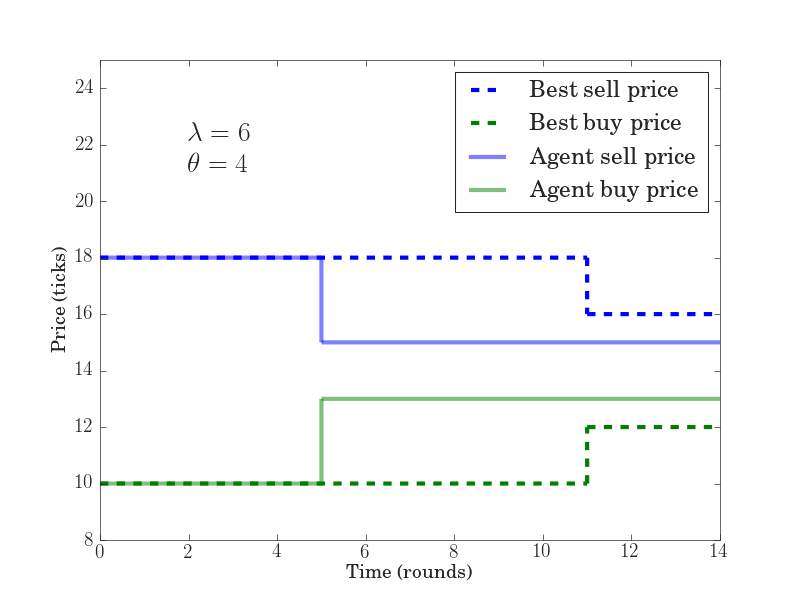
\includegraphics[width=0.5\textwidth]{21_scatter_plots/d9/b.png}}
\caption{Scatter plots of fitness measures in experiment \dnine. }
\label{figure:scatter_log_transform}
\end{figure}

Scatter plots are probably among the most rudimentary of techniques for data analysis, yet they can be incredibly informative, especially when the data that is visualized is low-dimensional.
The two plots in figure make two things clear. First of all, extreme values occur in \stdev. Even log scaling does not seem to fix this problem entirely. Second of all, XXXissue109XXX

The high correlation between \stdev and \overshoot can be interpreted in two ways. 
The sparsity of points with extreme values shows that it rarely


\begin{enumerate}
\item It rarely happens that a market has a large overshoot, and then returns to a stable state (large \overshoot, small \stdev)
\item 
\end{enumerate}

For the purposes of data analysis, the high correlation between \stdev and \overshoot means that it is possible to reduce the number of dimensions in the fitness space from four to three without loosing any significant classification power. This can be done by discarding either \stdev or \overshoot. %, or by using PCA to find the three dimensional projection with the highest variance/


\begin{figure}
\subcaptionbox{$\log \stdev$ vs. $\log \roundstable$ vs. \timetoreachnewfundamental}
[0.49\linewidth]{\includegraphics[width=0.5\textwidth]{103_scatter_manual_outlier/d9/d.png}}
\subcaptionbox{\roundstable vs. \timetoreachnewfundamental vs. \stdev}
[0.49\linewidth]{\includegraphics[width=0.5\textwidth]{103_scatter_manual_outlier/d9/c.png}}
\caption{}
\label{fig:}
\end{figure}


\subsection{Calculating statistics for outliers}

\begin{table}
	 \centering
	 \begin{tabular}{lrrrr}
	\toprule
	{} &  \overshoot > 10 (mean) &  \overshoot > 10 (mean) &  \overshoot > 10 (std) &  \overshoot > 10 (std) \\
	\midrule
	\sclatencymu                &                    73.8 &                    21.2 &                   21.2 &                   13.2 \\
	\sclatencys                 &                     5.2 &                     9.6 &                    9.6 &                    5.7 \\
	\scthinkmu                  &                    64.3 &                    24.3 &                   24.3 &                   13.6 \\
	\scthinks                   &                    11.4 &                    10.2 &                   10.2 &                    5.6 \\
	\sctimehorizonmu            &                  1804.5 &                  2134.1 &                 2134.1 &                 1444.1 \\
	\sctimehorizons             &                  1413.2 &                  1024.0 &                 1024.0 &                  629.2 \\
	\scwaitTimeBetweenTradingmu &                    29.9 &                    23.8 &                   23.8 &                   12.9 \\
	\scwaitTimeBetweenTradings  &                     3.6 &                     9.5 &                    9.5 &                    5.8 \\
	\ssmmlatencymu              &                    46.0 &                    29.9 &                   29.9 &                   14.7 \\
	\ssmmlatencys               &                     4.6 &                     8.8 &                    8.8 &                    5.0 \\
	\ssmmthinkmu                &                    37.6 &                    27.0 &                   27.0 &                   14.2 \\
	\ssmmthinks                 &                     0.9 &                    10.0 &                   10.0 &                    6.0 \\
	\bottomrule
	\end{tabular}
	\label{LABEL}
	\caption{CAPTION}
\end{table}